\chapter{Testing}

\section{User Interface Tests}
Die Domain Klassen der RadioTour Applikation enthalten wenig bis gar keine Logik. Aus diesem Grund wird auf herkömmliche \glspl{junit} verzichtet. Als Ersatz dazu werden zwei Ansätze zum testen des User Interfaces verwendet. Zum einen ist ein Testprojekt mit Hilfe des Test Frameworks Robotium vorhanden. Anderseits wird der Android SDK interne Monkey verwendet.
\subsection{Robotium Testprojekt}
 Mit Hilfe von Robotium werden Klicks sowie Texteingaben an die Applikation gesendet. Das Testprojekt ist deshalb eine Form des automated User Interface Testings. Wird das Testprojekt gestartet führt es folgende Aufgaben durch:
\begin{itemize}
\item Starten der Applikation\\
Das Testprojekt startet die Applikation und wartet das erfolgreiche Ausblenden des Splashscreen ab
\item Importieren von Fahrern\\
Falls die Applikation keine Fahrerinformationen enthält,navigiert das Testprojekt mit Hilfe von gesendeten Klicks zum Admin Bereich der Applikation und wählt das richtige Import csv-File aus.
\item Gruppieren von Fahrern\\
Das Testprojekt wählt zwei Fahrer aus und setzt sie an die Spitze. Dabei wird getestet ob nach dem Auswählen wirklich zwei Fahrer ausgewählt sind und nach dem Gruppieren wieder keine.
\item Testen der Gruppen Konsistenz\\
Es wird getestet ob jeweils nur eine Gruppe mit der Bezeichnung "`Spitze"' sowie nur eine mit der Bezeichnung "`Feld"' vorhanden ist
\item Neustart der Applikation \\
Das Testprojekt schliesst die Applikation und startet sie neu. Dabei wird überprüft ob der Gruppenstand vor dem Schliessen der Applikation derjenigen nach dem Neustart entspricht
\item Neues Maillot erstellen\\
Mit Hilfe der gesendeten Klicks wird ein neues Maillot erstellt und ein Fahrer als Träger dieses Maillots eingestellt. Darauf wird überprüft ob zum angegeben Fahrer der Eintrag zum Maillot vorhanden ist.
\item Neues Spezialklassement erstellen\\
Das Testprojekt navigiert zum Spezialklassement Bereich und erstellt dort ein neues Spezialklassement sowie eine neue Wertung. Zu dieser Wertung werden die Gewinner eingegeben. Darauf wird überprüft ob die Bonuspunkte sowie Bonuszeit bei den angegebenen Fahrern korrekt eingetragen sind.
\item Löschen der oben erstellten Objekte \\
Die in den oben aufgeführten Aufgaben erstellten Objekte werden - bis auf die Fahrer -  gelöscht. Nach dem Löschen überprüft das Testprojekt ob sich alle Fahrer wieder in der Ausgangslage befinden.
 

\end{itemize}

\subsection{Android Monkey}
Der Android Monkey ist ein Kommandozeilentool welches auf jedem Android Gerät sowie dem Emulator ausgeführt werden kann. Das Tool sendet pseudo-zufällige Benutzer Events in schnellstmöglicher Abfolge an das System welches getestet wird. Dadurch werden Fehler im User Interface unabhängig von der darunter liegenden Logik aufgedeckt. Im Zusammenspiel mit dem Robotium Testprojekt kann deshalb, sofern beide Testmethoden erfolgreich durchlaufen, davon ausgegangen werden, dass die \textit{RadioTour} Applikation sich stabil und erwartungsgemäss verhält.

\section{Feldtest}

Um die Benutzerfreundlichkeit und den Mehrwert der Applikation im Vergleich zur bisherigen Web Applikation zu ermitteln ist ein Feldtest unabdingbar. Es gab die Möglichkeit die \textit{RadioTour} Applikation in einem Berner Fahrrad Rennen zu testen. Bei der Berner Rundfahrt\footnote{Berner Rundfahrt \url{http://www.berner-rundfahrt.ch}} bot sich der  \textit{RadioTour Speaker} der Berner Rundfahrt, David Loosli\footnote{David Loosli, ehemaliger profi Radrennfahrer und \textit{RadioTour Speaker} der Berner Rundfahrt} ,an die Applikation zu testen. In einem ersten Treffen wurden die grundlegenden Funktionen der Applikation und die Bedienung erklärt. Weiter ist ein Ausschnitt aus einem fiktiven Rennen durchgespielt worden, wobei eine Person den \gls{chronofunk} simulierte. Ein kurzer Auszug aus der vorbereiteten Situation ist unten aufgeführt.

\begin{itemize}
\item alle Fahrer sind importiert und das Rennen beginnt jetzt
\item Rennzeit wird gestartet
\item \textit{Chronofunk:} Fahrer 4 \& 17 von Beginn an, an der Spitze
\item \textit{Chronofunk:} Bereits 1:07 Vorsprung
\item \textit{Chronofunk:} 31 hat ein defektes Rad und muss raus
\item \textit{Chronofunk:} 8, 83 \& 34 fallen hinter das Feld mit einem Rückstand von 4:31
\end{itemize}

Der vollständige Usability Test sowie der Testlauf an der \textit{Berner Rundfahrt} mit den Rückmeldungen von Herrn Loosli sind im Anhang \ref{ref:usability} zu finden.

Mit den Erfahrungen und den Rückmeldungen aus diesem Event konnte das Endprodukt massiv verbessert werden. Die wesentlichen Punkte die für die Weiterentwicklung verwendet wurden sind:
\begin{itemize}
\item TimePicker Nummern (Auswahl des Rückstandes einer Gruppe) sind zu klein (Korrektur siehe Abbildung \ref{fig:timepicker})
\item nur die Fahrer welche aufgegeben haben oder nicht erschienen sind sollen ausgegraut werden (Vorschlag in Abbildung \ref{fig:riderpicker})
\item ein Fahrer kann folgende Status haben:
\begin{itemize}
\item im Rennen / aktiv
\item nicht gestartet
\item ausgeschieden
\end{itemize}
\item Rennzeit und Kilometer sind nach einem Absturz der Applikation noch verfügbar
\end{itemize}

\begin{figure}[h!]
\caption{TimePicker - Auswahl eines Zeitrückstandes}
\label{fig:timepicker}
\centering
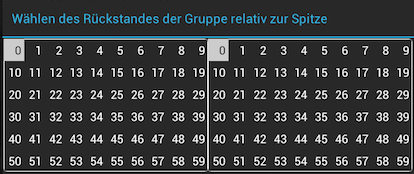
\includegraphics[scale=0.8]{05bericht/images/timepicker.png}
\end{figure} 
Besonders zu hervorheben ist an dieser Stelle, dass Herr Loosli entgegen den Erwartungen die Fahrer, welche in einer Gruppe eingeteilt sind (z.B. Spitze) nicht ausgegraut haben möchte. So entstand der, in Abbildung \ref{fig:riderpicker} dargestellte Entwurf.

\begin{figure}[h!]
\caption{RiderPicker - Auswahl von Fahrern}
\label{fig:riderpicker}
\centering
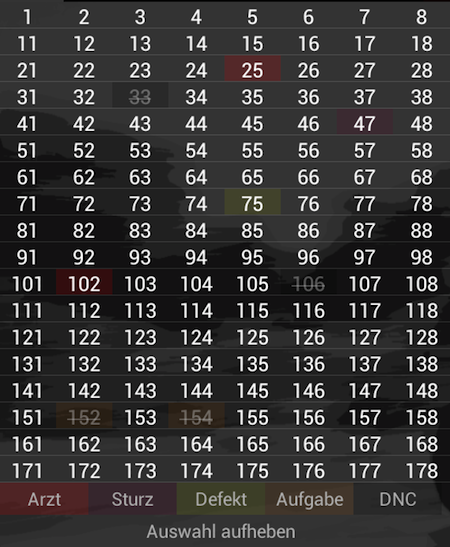
\includegraphics[scale=0.5]{05bericht/images/riderpicker.png}
\end{figure}

Die Abbildung \ref{fig:riderpicker} zeigt eine Situation, bei der die Fahrer 33 und 106 nicht gestartet sind und die Fahrer 152 und 154 aufgegeben haben. Diese Fahrer sind farblich markiert und durchgestrichen. Die weiteren Farben entsprechen den besonderen Ereignissen; Arzt, Sturz oder Defekt eines Fahrers bzw. eines Fahrrads.
